% 9 variables in here:
% h_1 = 10.0, h_2 = 10.0, h_3 = 10.0, ux_1 = 0.0, ux_2 = 0.0, ux_3 = 0.0, uy_1 = 0.0, uy_2 = 0.0, uy_3 = 0.0
\begin{figure}[ht]
\centering
  \quad \subfloat[] {
    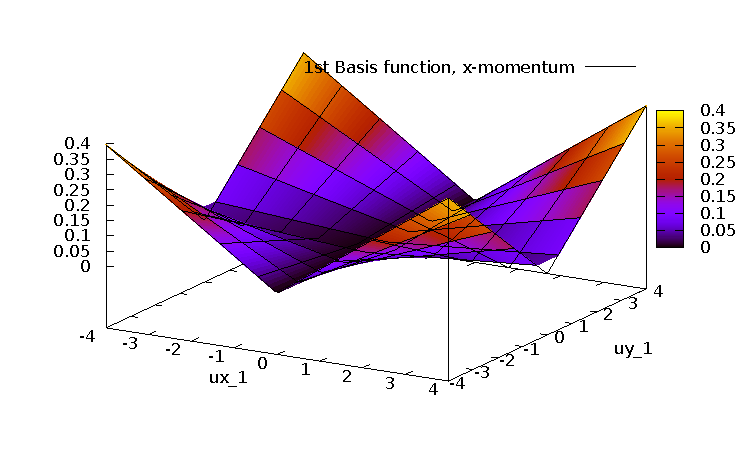
\includegraphics[scale=\zoomfactor]{{{standardwerte_nach_ux1_uy1_ord1/10.0_10.0_10.0_x_0.0_0.0_y_0.0_0.0f00}}}
  }
  \quad \subfloat[] {
    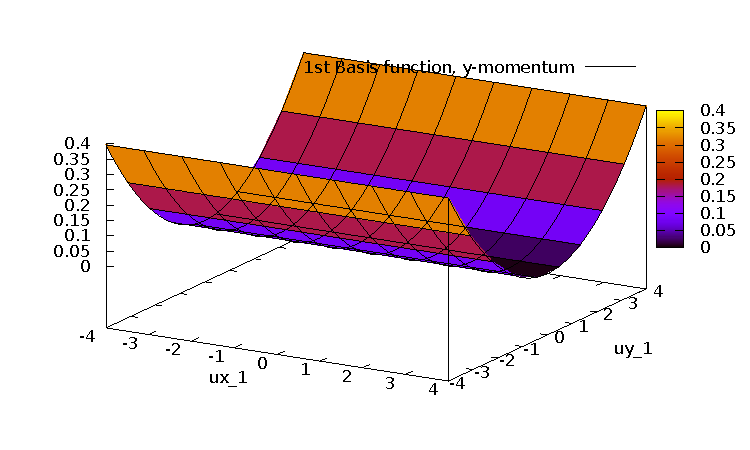
\includegraphics[scale=\zoomfactor]{{{standardwerte_nach_ux1_uy1_ord1/10.0_10.0_10.0_x_0.0_0.0_y_0.0_0.0f01}}}
  }
  \quad \subfloat[] {
    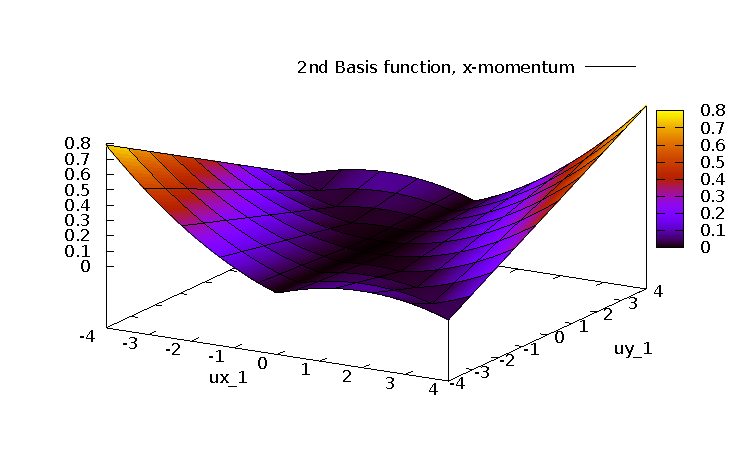
\includegraphics[scale=\zoomfactor]{{{standardwerte_nach_ux1_uy1_ord1/10.0_10.0_10.0_x_0.0_0.0_y_0.0_0.0f02}}}
  }
  \quad \subfloat[] {
    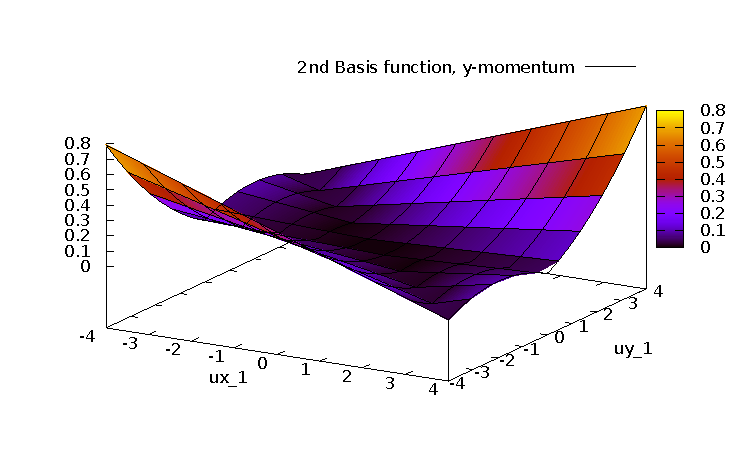
\includegraphics[scale=\zoomfactor]{{{standardwerte_nach_ux1_uy1_ord1/10.0_10.0_10.0_x_0.0_0.0_y_0.0_0.0f03}}}
  }
  \quad \subfloat[] {
    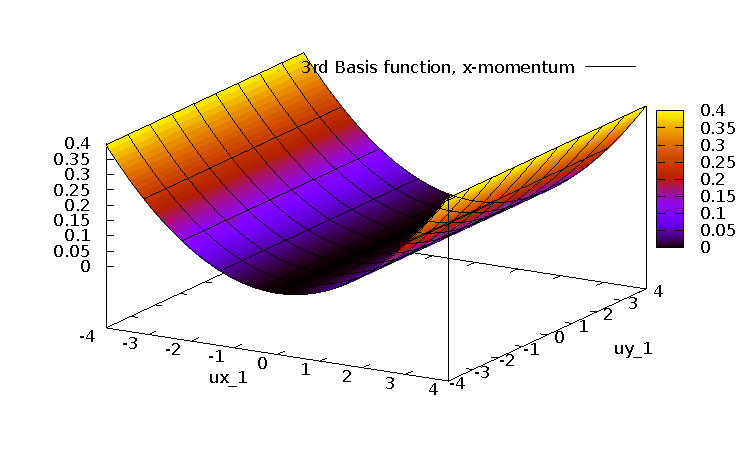
\includegraphics[scale=\zoomfactor]{{{standardwerte_nach_ux1_uy1_ord1/10.0_10.0_10.0_x_0.0_0.0_y_0.0_0.0f04}}}
  }
  \quad \subfloat[] {
    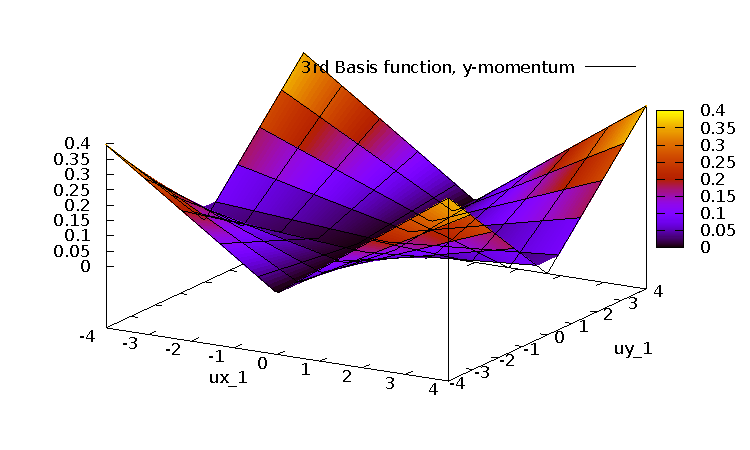
\includegraphics[scale=\zoomfactor]{{{standardwerte_nach_ux1_uy1_ord1/10.0_10.0_10.0_x_0.0_0.0_y_0.0_0.0f05}}}
  }
\caption{Basis functions of order 1. Variables $u_{x,1}$ and $u_{y,1}$ are the axes of the plots. All height values are set to 10, all remaining momentums set to 0. Note that $SE_x^1$ looks like $SE_y^3$. Also note the symmetry between some other plots: $SE_x^3$ corresponds to $SE_y^1$, mirrored by the plane $u_{x,1}=u_{y,1}$. The plots for the second basis functions are mirrored by that plane.}
\label{fig:standardwerte_nach_ux1_ux2_ord1}
\end{figure}

%%% Local Variables:
%%% TeX-master: "../results.tex"
%%% End:
